\section{Mining Power Oracle}

The notion of variable difficulty in blockchain protocols stems from the fact that the mining power of the network changes with time. In the Bitcoin Backbone model, this is treated by considering the dynamic number of parties of the protocol $n_j$ for every epoch $j$. While legacy blockchain protocols use the blockchain growth rate to approximate mining power available on the network, we observe that the notions of measuring mining power available on the network and the blockchain protocol itself are two distinct concepts. However, on the one hand, measuring mining power can be done by observing the blockchain; on the other hand, the blockchain protocol itself can adjust its parameters by looking at the changing mining power.

Nevertheless, we observe that measuring mining power is a distinct primitive which is utilized by blockchain protocols and it can be realized via different mechanisms than measuring chain growth. The primitive itself can be modelled as a functionality which allows parties to query the currently available mining power in the form of an oracle. The ideal oracle returns the exact current mining power of the network, while a realistic oracle returns an approximation of the current mining power within a known margin of error. In our treatment of variable difficulty protocols, we assume that the mining power oracle is realized in one way or another and build our protocol on top of it.

In this section, we propose a different mechanism through which current mining power can be measured. The protocol works as follows and is agnostic of the concept of a blockchain. Whenever an honest party successfully queries the mining random oracle to generate a block, it diffuses that block on the network as an indicator of mining power available. (TODO: what target is considered in this process?) When an honest party receives such a block, it remembers it so that it can use it to count the current mining power available on the network. This caching avoids honest parties counting incoming blocks multiple times. Each block received in this protocol is marked with the round during which it was received. When an honest party receives such a block from the rest of the network, they relay it to the rest of the network. This ensures all honest parties will receive it with at most one round of delay. Subsequently, the honest party calculated a weighted average of the block counts received to extract an estimate of the currently available network mining power. The weighted average is taken by applying a normal distribution weight based on the block timestamps. By taking the weighted average, the honest parties will arrive at a similar approximation of the currently available mining power. The weighting function is shown in Figure~\ref{fig:mining-power}.

\begin{figure}[h]
\begin{center}
  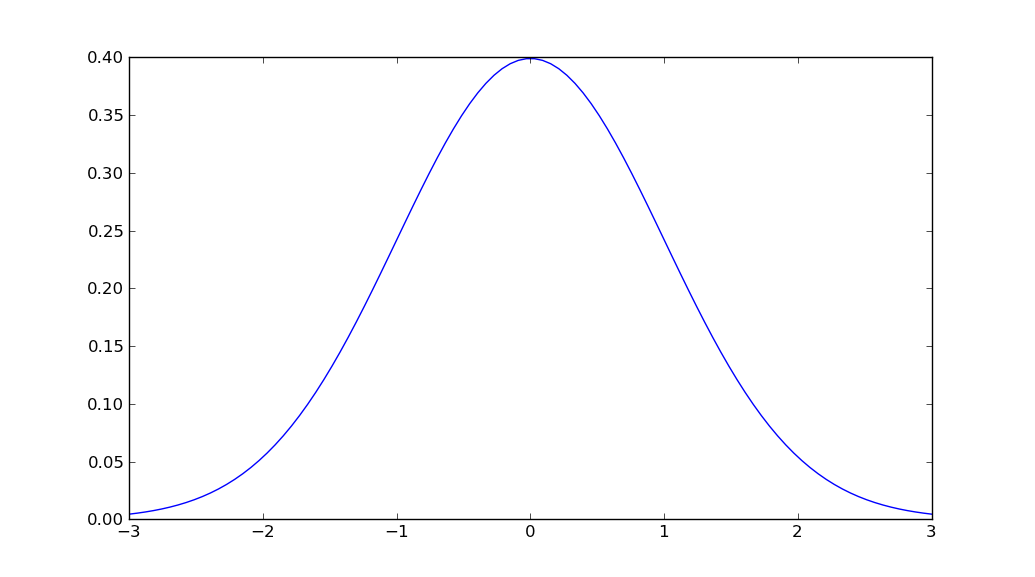
\includegraphics[width=1\columnwidth]{figures/normal.png}
  \caption{The normal distribution is used to weight block counts to extract mining power.}
  \label{fig:mining-power}
  \end{center}
\end{figure}
